\section[M3: QVTo]{M3: QVTo - Modelltransformation}
\begin{frame}{QVTo - Modelltransformation}
	\centering
	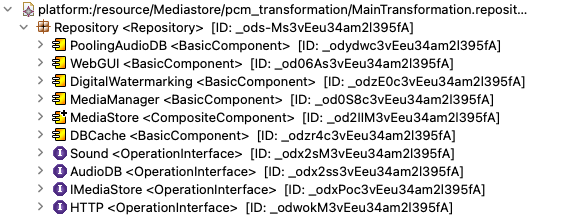
\includegraphics[height=40mm]{figures/qvto.png}
\end{frame}

\begin{frame}{Entwurfsentscheidungen und Probleme bei der Modelltransformation}
	\begin{enumerate}
		\item Verwendung von intermediate-Objekt \texttt{TRole} zur Repräsentation von unterschiedlich existierenden Konzepten im Meta-Modell
		\begin{itemize}
			\item Interface- und Communicator-Konzept ist in Palladio anders umgesetzt
			\item Unterschiede: Modellierung in Metamodell als Property und in Palladio als Klasse
		\end{itemize}
		\item Ausnutzen der Vererbungshierarchie in Metamodell
		\begin{itemize}
            \item Abstraktes Mapping: Mapping von abstraken Klassen mit Hilfe von polymorphen Disjunct-Mapping
            \item Für Vererbungshierarchien auf Source-/Target-Seite $\rightarrow$ zusätzliche Verwendung für Mapping der Datentypen
        \end{itemize}
	\end{enumerate}
\end{frame}